
 \documentclass[preprint,12pt]{elsarticle}


\usepackage{float}
\usepackage[english]{babel}
\usepackage[utf8x]{inputenc}
\usepackage{amsmath}
\usepackage{graphicx}
%\usepackage[colorinlistoftodos]{todonotes}
\setcitestyle{square}
\usepackage{verbatim}

\journal{Expert Systems with Applications}

\begin{document}

\begin{frontmatter}

\begin{comment}
%%Research highlights
\begin{highlights}

\item Combination of news and stock market features for analyzing stock market movements
\item Applying Natural Language Processing techniques like LDA, Tf-Idf and Sentiment Analysis for Feature Extraction from news data
\item A method to partition the dataset for training has been proposed which resulted in 97 percent accuracy
\item Machine Learning algorithms are able to learn better when news features have been added to the stock market data
\end{highlights}
\end{comment}

\title{Forecasting News Driven Stock Market Movements using ML and NLP Techniques}


\author{Nippani Abhinav, A Venkata Sravan Bharadwaj, Dr. Nivedita Sinha }

\address{Birla Institute of Technology and Sciences - Pilani, Hyderabad Campus, India}
\address[Nippani Abhinav]{f20160278@hyderabad.bits-pilani.ac.in}
\address[A Venkata Sravan Bharadwaj]{f20160400@hyderabad.bits-pilani.ac.in}
\address[Dr. Nivedita Sinha]{nivedita.sinha@hyderabad.bits-pilani.ac.in}

\begin{abstract}
%% Text of abstract
This paper tries to formulate a method to predict the direction of a stock market index (NIFTY 50) on a day-to-day basis. This is done using News Headlines and a few Stock Market features as inputs to an ensemble of Machine Learning and Natural Language Processing Algorithms. 
Two datasets are considered - the first considers a combination of Stock Market features and News Headlines as input while the second model considers only the Stock market features without considering News.
The models combine LDA (Latent Dirichlet Allocation), Tf-Idf, Sentiment Analysis which are natural language processing techniques and XGBoost, Random Forest, Decision Tree and KNN which are machine learning algorithms to predict the direction of the index. Data has been considered from 2010 to 2018. 
Two different methods of partitioning the dataset have been considered for evaluating the model. The first one calculates the accuracy using a simple train-test split or grid search. The second method for splitting used is introduced in this paper which calculates the accuracy by training the data using windows on a rolling basis. While a maximum of 70 percent accuracy has been achieved using the first method, the second method gives a maximum of 97 percent accuracy.
These results obtained in this paper prove that the method used is indeed a novel way to approach the influence of news on stock market movements.

\end{abstract}

%%Graphical abstract
%%\begin{graphicalabstract}
%\includegraphics{grabs}
%%\end{graphicalabstract}



\begin{keyword}
Machine Learning, Natural Language Processing, Stock Market, Latent Dirichlet Allocation(LDA),Random Forest, XGBoost

\end{keyword}

\end{frontmatter}

%% \linenumbers
%\pagebreak
%% main text
\section{INTRODUCTION}

Over the years, the techniques used for analyzing stock market movements have been rapidly evolving because of reasons like increase in access to data, computational power to process this increase in data. The applications of machine learning and natural language processing techniques have had a tremendous impact on stock market trading over the previous decade due to advancements in artificial intelligence as a whole.

The stock market is viewed as a complex environment, where the stock movements are impacted by a varied number of factors. Millions of organized and unstructured information are created day by day around the world making it even more complex to analyze. Historically, two methods have been adopted for analyzing stock market data: fundamental analysis and technical analysis.

Fundamental Analysis is a method of estimating the intrinsic value by analyzing the financials of a company by examining the balance sheet, income statement, etc which are publicly disclosed by the company. This doesn't impact stock market movements on a daily basis but it is the major reason for impacting the stock price in the long run. Technical Analysis is a method of estimating the stock market movements on a short term basis using various price patterns, charts, technical indicators, etc which might not have any direct relations with the financials of the company.


Although these historical techniques have been successful to an extent, there is a huge scope for improvement as the market is becoming even more challenging in the current times. In the recent past, many machine learning techniques have been applied for analyzing the stock market data. These techniques have been successful in predicting the future prices with considerable accuracy. With increasing research and better computational devices available, machine learning techniques have also been evolving manifolds. Tree based methods are performing better compared to conventional methods like logistic regression. Ensemble learning techniques like bagging, stacking and boosting which combine several machine learning and deep learning techniques have also been successfully used to improve the prediction accuracies and significantly reduce losses.

The buyers and sellers decide the price of a stock in the market. This implies that the law of supply and demand determines the stock prices. The demand increases if the investors feel that the company will perform well and the demand decreases if the investors feel otherwise. In other words, the stock price can be taken as a measure of the future performance of a company. However, many other factors can also affect the future performance of a company. There are various theories about to stock prices in literature. Among these, Efficient Market Hypothesis (EMH) \cite{emh} is the most representative.It states that the market price reflects the value accurately. The market price responds only to new information which contains historical prices, public and private information. According to how the information is reflected, EMH is divided into three categories: Weak, Semi and Strong. Since majority of the mature stock markets are weak-form efficient markets, the stock prices could be considered reflective of current information. This is where news comes in. Analyzing news and correlating it with the stock prices has a huge potential. This the reason why many studies have been conducted on trying to predict the stock prices using financial news. 

In almost all of the studies on analyzing the trend of stock prices, news and stock market features like high, open, close,etc were analyzed separately. The news was classified according to its sentiment which helped in predicting the trend of the stock prices for example by using twitter feeds \cite{text_1}; news headlines\cite{text_2}. Many of these methods have been summarized in \cite{text_3}. The stock market features were used to predict the future prices of the stock market by using machine learning techniques for example using statistical techniques \cite{stock_1}; disparate data sources \cite{stock_2} and ensemble methods \cite{stock_3}.
This paper tries to combine both these methods by using natural language processing techniques to process the textual data from news into numerical data. This data along with the data from stock market features is then used to predict the prices using machine learning algorithms, and its accuracies are compared.

\section{ALGORITHMS }

\subsection{LDA}
Latent Dirichlet Allocation \cite{lda} is a popular Topic Modelling technique. Topic Modelling is the task of classifying a paragraph or dataset automatically into a set of categories.

LDA assumes that each dataset is a set of documents or sentences (rows) and each document or sentence is a set of different categories. So, each sentence will be categorized into a percentage of each of the categories. Most of the words are captured by these imaginary categories.

Assuming this generative model for a collection of documents, LDA then tries to backtrack from the documents to find a set of categories that are likely to have generated the collection.

In each document, randomly assign each word to one of the ‘K’  categories. This already gives both category representations of all the documents and word distributions of all the categories (although not very good ones).
For each word w in document d,for each category t, compute two things: 
\begin{itemize}
\item    p(category t | document d) = the probability of words assigned to category t in document d 
\item   p(word w | category t) = the probability of assignments to category t which come from word w over all documents.
\end{itemize}
Reassign w to a new category, where the newly chosen category t with probability p(category t | document d) * p(word w | category t) (= probability that word w is generated by category t). Basically, in this step, it is assumed that all assignments to the categories except for the current word are correct. The assignment to the current word is then updated using the model of how documents are generated. The assignments to the words stabilize on repeating the previous step many times. These stabilized assignments are then used to estimate the mixture of each category in each document (proportion of words assigned to each category within that document) and the words associated to each category (proportion of words assigned to each category overall).

\subsection{Tf-Idf}

Tf-Idf stands for Term frequency-Inverse document frequency. The Tf-Idf Score is a statistical measure and is used to evaluate how important a word is to a document in a collection or corpus. TF-IDF quantifies the relevance of each word in the dataset. This method is often used in information retrieval and text mining. Tf-Idf can be successfully used for filtering stop-words \cite{tfidf_1,tfidf_2,tfidf_3} in various subject fields including text summarizing and classification.

Tf-Idf is calculated by multiplying two terms: Term Frequency (TF) and Inverse Document Frequency(IDF).

\subsubsection{Term Frequency (TF)}
Term Frequency (TF) is a measure of how frequent a term occurs in a document. Let the number of times a term 't' appears in a document be represented by '$n_d$' and the total number of terms in the document be represented by 'n'.
\begin{equation}
TF(t) = \dfrac{{n_d}}{n}
\end{equation}
\subsubsection{Inverse Document Frequency (IDF)}
It is a measure of how important a term is. While computing TF, all terms are considered equally important. However it is known that certain terms, such as "is", "of", and "that", may appear a lot of times but have little importance. Thus, to give more importance to the rare terms and reduce the importance of more frequent terms, IDF is computed.The higher the score, the more relevant that word is in that particular document. Let the total number of documents be represented by 'd' and the number of documents with term 't' in it be represented by '$d_t$'.
\begin{equation}
IDF(t) = log_e(\dfrac{d} {{d_t}})
\end{equation}

\subsection{Decision Tree}

CART stands for Classification and Regression Trees and is a type of decision tree algorithm. It is a recursive algorithm which creates a tree used for supervised classification tasks.

Each node in the Decision Tree is split in such a way that the Gini impurity of the children of that node is minimized. Gini Impurity is a metric used to define how homogeneous a node is. If all samples of a node belong to the same class, Gini Impurity is zero whereas a node with many samples will have higher value. The Gini Impurity of n training samples with k classes is given by 
\begin{equation}
G = 1 - \sum_{k = 1}^{n}p_k^2
\end{equation}
The Decision Tree is formed by splitting the nodes recursively in the above described way till the maximum depth is reached.In a Decision Tree, the root node has highest Gini Impurity and the subsequent nodes will have lower Gini Impurities. Hence, each node represents a rule. For each test case, the output is predicted using these predefined rules.


\subsection{Random Forest}
Random Forest \cite{random_forest} is a Bagging (Bootstrap Aggregating) ensemble algorithm. Bagging algorithms use many “Decision tree” algorithms which separately classify the data and predict the results. 

Every decision tree in the multiple decision trees of random forest separately classify the data based on a best split criteria (unique for each tree) of a random set of the training data. Gini index values determine the best split criteria. For each node in the tree, gini index measures the variation from the perfect accuracy. The Random Forest algorithm works by first randomly selecting features from the total number of features. Calculate the best split criteria for a node. Split this node into daughter nodes using best split criteria. Similarly split these daughter nodes further till the maximum number of levels is reached. Now a tree is formed. Create many such trees to form a forest. The Model is now created. For each test case, predict the outcome for each tree. The most common output from the set of all defined trees will be taken as the final output


\subsection{XGBoost}

XGBoost stands for eXtreme Gradient Boosting. XGBoost is an ensemble of gradient boosting decision tree algorithms.  In boosting, models are added sequentially to improve upon the errors of the previous models till the error is nil or an improvement cannot be done. The new models which are created try to predict the residuals of previous models and then these are added together to make the final prediction. The loss is minimized when adding the new models using gradient descent algorithm  and hence the name gradient boosting. 

XGBoost is a supervised learning method that is based on function approximation by optimizing specific loss functions as well as applying several regularization techniques.

\subsection{KNN}

KNN stands for K-Nearest Neighbours. It is an instance based learning algorithm and has many applications in pattern recognition and data mining. It falls into the category of Supervised learning algorithm and is commonly used for classification tasks. KNN is easily interpretable and is a fast algorithm.

K Nearest Neighbour algorithm assigns a class to a datapoint/instance based on the classes of k nearest/similar points/instances to that datapoint/instance The Similarity metric is given by a distance metric between the two instances considered. The most popularly used metric is the Euclidean distance which is given by the following formula:
\begin{equation}
d(x,x') = \sqrt{ {{(x_1 - x_1')}^2} + {{(x_2 - x_2')}^2} + \ldots + {{(x_n - x_n')}^2} }
\end{equation}
A few other commonly used similarity metrics include Manhattan, Chebyshev and Hamming distance.The KNN algorithm works in the following way:

Choose hyper parameters k and distance metric d. For each new observation ‘x’  in the data , calculate the distance ‘d’ between ‘x’ and each other observation. Choose ‘k’ observations which are the closest to ‘x’. Let the set of these ‘k’ points be called ‘A’. Calculate the conditional probability for each class given these ‘k’ points using the formula given below (I(x) returns 1 when the argument is true and 0 otherwise). ‘x’  gets assigned to the class with the highest probability.

\begin{equation} 
P(y = j|X = x) = \dfrac{1}{K}\sum_{i\in A} I({y^{(i)}} = j) 
\end{equation}

\section{METHODOLOGY}
As explained, this paper tries to combine features from news and stock to try and predict the future prices of stock market. 

The features from News are obtained by preprocessing a public dataset of daily news headlines (obtained from a public dataset on Kaggle title News Headlines of India) which have been collected for the period 2010 to 2018.

\begin{figure}[H]
\centering
\includegraphics[width=390pt,keepaspectratio]{News_Preprocessing_Flowchart.eps}
\caption{\label{fig:news_preprocessing} Preprocessing News into Numerical Features}
\end{figure}



The daily news headlines need to be preprocessed into numerical features for the model to easily understand. This is done with the help of Natural Language Processing(NLP) techniques. As depicted in Figure~\ref{fig:news_preprocessing}, the daily news headlines need to be cleaned for further preprocessing. Then, the stop words or unnecessary words need to be removed from this dataset using Tf-Idf. The topics are then identified using LDA and then each headline is assigned its importance to these topics. These values are then multiplied with sentiment polarity values using Sentiment Analysis.The sum of these values for each topic per day is then taken as the final features from the news headlines.

\subsection{Cleaning News Dataset}

The News Dataset obtained has to be cleaned for further operations. Remove new line characters, distracting single quotes, Emails, Punctuation, Digits/Numerals, Extra White space and convert all words to Lowercase.

\subsection{Filtering out Stop words}

On the obtained preprocessed news dataset TF-Idf algorithm is applied to filter out the stop words. The Tf-Idf Scores are obtained for each word in the dataset. The words which don’t have any importance are added to the stop words list(Words which need to be removed from the document).

The Stop words list is taken from two sources. The first is a predefined list of stop words available in NLTK Library. The second list of stop words is taken from the words filtered after applying Tf-Idf Algorithm. The obtained stop words are then removed from the entire dataset.

\subsection{Sentiment Analysis}

In this step, the sentiment value of each headline in the dataset is calculated. Here the sentiment value quantifies the polarity of the Headline, i.e , how much positive or negative each headline in the dataset is.

\subsection{Segmentation into Topics}

This cleaned news dataset is divided into categories using Topic Modelling. One of the algorithms for Topic Modelling is Latent Dirichlet Allocation(LDA). This LDA model has been used to divide the news dataset into categories.

The LDA Model takes the entire dataset and number of categories as inputs and returns sets of keywords for each category

\subsection{Coherence Score and Tuning the LDA Model}

The efficiency of the model is quantified by calculating the Coherence Score. Coherence Score is a measure of the semantic similarity between high scoring words of a topic.The range of coherence scores is between 0 and 1 with a value close to 0 implying no similarity or coherence between the words in a topic and a higher values represent higher degree of similarity or coherence.

The parameters of the LDA model are number of Categories required, Dirichlet hyper parameter alpha ( document-topic density) and Dirichlet hyper parameter beta (word-topic density)

All the above parameters are iterated and the Coherence Score is calculated for each of the iterations. The model with the highest Coherence Score is then selected. The Obtained Coherence Scores are shown in the Figure~\ref{fig:coherence_scores}.

\begin{figure}[H]
\centering
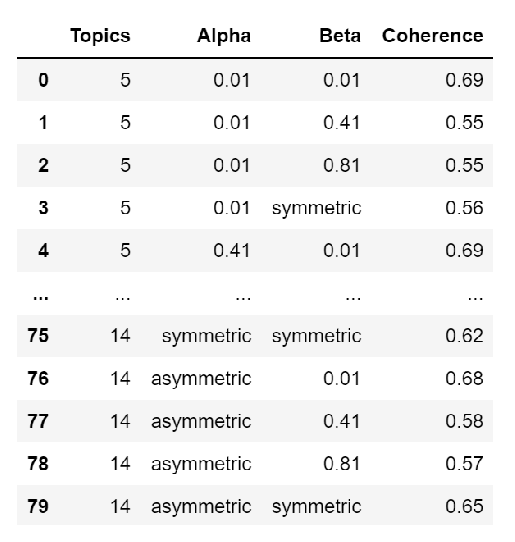
\includegraphics[width=8cm,height=20cm,keepaspectratio]{Coherence_Scores.eps}
\caption{\label{fig:coherence_scores} Coherence Scores}
\end{figure}


The top keywords for each category have now been obtained using the optimal LDA model.The percentage contribution of each topic towards each headline are numerical. This gives a dataset with each headline vs contribution of each topic in that headline.

\subsection{Creating Final News Dataset}

Now the numerical dataset is obtained which measures the contribution of each topic/category towards each headline using LDA.However, the polarity of each headline has yet to be included in this. This is where the previously calculated sentiment values come in. 
The Sentiment Values are multiplied to each row in the numerical dataset.
Now, the dataset represents the topics as well as the sentiment polarity of each headline.
However, the final dataset should be representative of each day and not of each headline. To do this the sum of the values obtained for headlines on each day is considered. This helps in quantifying the volume of news obtained as well as the net polarity of each category of that day will be the outcome of this step.

The news dataset is now preprocessed and is easily interpretable by the model. The news features and stock features should now be combined to form a single dataset. 

\subsection{Preprocessing Stock Dataset}

The Stock Dataset has the following features: High, Low, Open, Close, Close one day prior and Volume of the index(NIFTY 50).


The Percentage Differences of these features (Percentage Returns) are calculated and replaced in the dataset. This is done as the absolute values vary over the years and Returns would be better values for the model to learn.

\subsection{Combining the Datasets}

Let the number of features in the stock dataset be N and the number of features or categories in the News dataset be M. The number of features in the combined dataset is M+N.Now, we have two datasets, Stock and Combined(Stock + News) as shown in Figure~\ref{fig:combining_datasets}.

\begin{figure}[H]
\centering
\includegraphics[width=10cm,height=10cm,keepaspectratio]{Combining_Datasets.eps}
\caption{\label{fig:combining_datasets} Combining News and Stock Features}
\end{figure}

\subsection{Output}

The direction of change in open values for next day as compared to current day value is considered as the output which needs to be predicted. The output is divided into two classes - Positive and Negative Directions. This is decided based on the Close Values. If the Close Value is higher on the predicted day as compared to the day before then that day or input is assigned as a Positive class. If the Close Value is lower on the predicted day as compared to the day before then that day or input is assigned as a Negative class.

\section{RESULTS}
The input and the output datasets are now formed. 2341 Data Points or Days out of which 1105 are positive, 1236 are negative. Since the dataset is equally balanced, Accuracy will be a good metric for evaluating the performance of the algorithms on the datasets.

The input datasets and output are now fed to various Machine Learning Models and the results are compared.The Machine Learning Models considered in this paper are XGBoost, Random Forest, Decision Tree and KNN.

Two different methods for splitting the datasets are used and the obtained metrics are compared among these methods. The methods used in this paper are Train-Test Split and Window based Roll Forward Partition.


\subsection{Train-Test Split / Grid Search}




Let X be the percentage of data to be trained. This implies 100-X percent of data will be predicted. The model will train on the X sized training dataset and predict the directions for the remaining 100-X test values. The percent of correctly predicted values gives the accuracy of the model. This is summarized in Figure~\ref{fig:train_test_split}.

\begin{figure}[H]
\centering
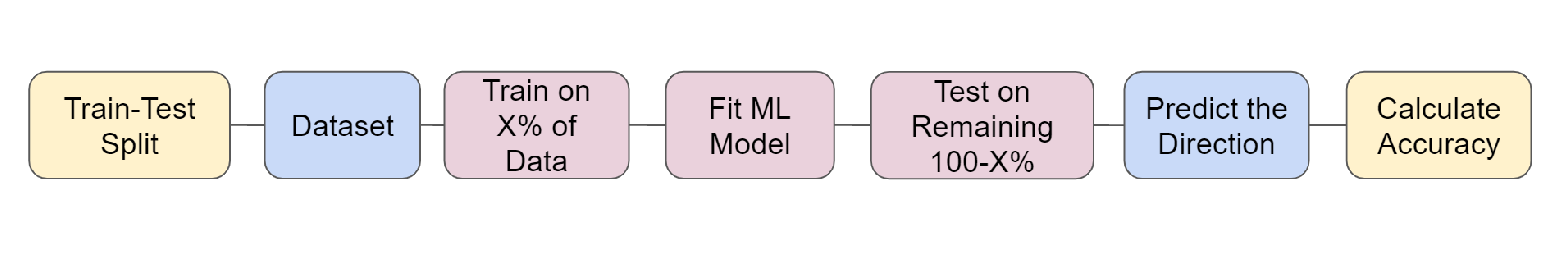
\includegraphics[width=390pt,keepaspectratio]{Train_Test_Split.eps}
\caption{\label{fig:train_test_split} Train Test Split}
\end{figure}


X is iterated from 60 to 85 and the obtained accuracies are plotted for both the datasets as shown in Figures~\ref{fig:XGBoost_Train_Test_Split}, \ref{fig:RandomForest_Train_Test_Split}, \ref{fig:DecisionTree_Train_Test_Split} and  \ref{fig:KNN_Train_Test_Split}. Each of these plots contain two lines which depict the different accuracies obtained for both the datasets for the above described splitting method. The red line represents the accuracies obtained for the combined(stock and news features) dataset whereas the blue line represents the accuracies obtained on training the models only on stock features.

\begin{figure}[H]
\centering
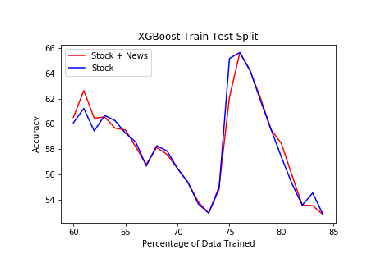
\includegraphics[width=10cm,height=10cm,keepaspectratio]{XGBoost_Grid_Search_Acc.eps}
\caption{\label{fig:XGBoost_Train_Test_Split} XGBoost Train Test Split}
\end{figure}

\begin{figure}[H]
\centering
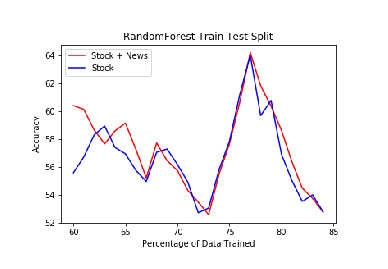
\includegraphics[width=10cm,height=10cm,keepaspectratio]{RandomForest_Grid_Search_Acc.eps}
\caption{\label{fig:RandomForest_Train_Test_Split} Random Forest Train Test Split}
\end{figure}

\begin{figure}[H]
\centering
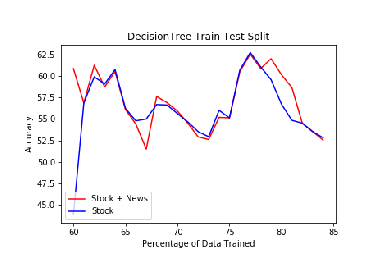
\includegraphics[width=10cm,height=10cm,keepaspectratio]{DecisionTree_Grid_Search_Acc.eps}
\caption{\label{fig:DecisionTree_Train_Test_Split} Decision Tree Train Test Split}
\end{figure}

\begin{figure}[H]
\centering
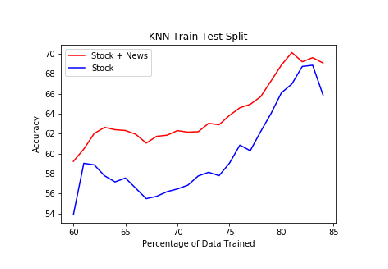
\includegraphics[width=10cm,height=10cm,keepaspectratio]{KNN_Grid_Search_Acc.eps}
\caption{\label{fig:KNN_Train_Test_Split} KNN Train Test Split}
\end{figure}

From Figures~\ref{fig:XGBoost_Train_Test_Split}, \ref{fig:RandomForest_Train_Test_Split}, \ref{fig:DecisionTree_Train_Test_Split} and  \ref{fig:KNN_Train_Test_Split} it is observed that KNN (70 percent), XGBoost (66 percent) and Random Forest (64 percent) have the highest accuracies followed by Decision Tree (62 percent). All the algorithms are able to learn the Combined(Stock+News) dataset better than the dataset with only Stock features. This is very clearly seen in KNN and marginally in other algorithms


\subsection{Window Based Roll Forward Partition}


To predict the direction of the index on a particular day, how many days prior to this date needs to be trained? The Window Train Partition aims to solve this question.

Let the number of days to be trained prior to the day to be predicted be X. If the model is trained on X days, then the ${(X+1)^{th}}$ day is predicted. This is done on a rolling basis.
If the number of days to be trained prior to the day to be predicted is X and the total number of days in the dataset is N, then the number of days which will be predicted is (N-X).

This means that there will be (N-X) models which predict the directions of these N-X days. The first model will train on 0-X days and predict the ${(X+1)^{th}}$  days. The second model will train on X+1 days and predict the ${(X+2)^{th}}$  day and so on. The final ${(N - X)^{th}}$  model predicts the Nth day. This is summarized in Figure~\ref{fig:window_based_roll_forward_partition}.

\begin{figure}[H]
\centering
\includegraphics[width=10cm,height=10cm,keepaspectratio]{Window_Based_Roll_Forward_Partition.eps}
\caption{\label{fig:window_based_roll_forward_partition} Window Based Roll Forward Partition}
\end{figure}

X is iterated from 60 days to 2000 days as windows and the obtained accuracies are plotted for both the datasets as shown in Figures~\ref{fig:XGBoost_window_training}, \ref{fig:RandomForest_window_training}, \ref{fig:DecisionTree_window_training} and  \ref{fig:KNN_window_training}. Each of these plots contain two lines which depict the different accuracies obtained for both the datasets for the above described splitting method. The red line represents the accuracies obtained for the combined(stock and news features) dataset whereas the blue line represents the accuracies obtained on training the models only on stock features.

\begin{figure}[H]
\centering
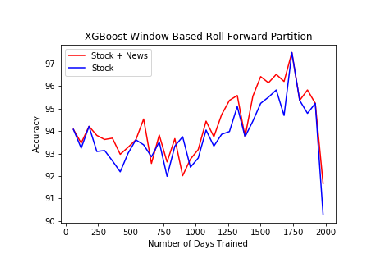
\includegraphics[width=10cm,height=10cm,keepaspectratio]{XGBoost_Window_Training_Acc.eps}
\caption{\label{fig:XGBoost_window_training} XGBoost Window Based Roll Forward Partition}
\end{figure}

\begin{figure}[H]
\centering
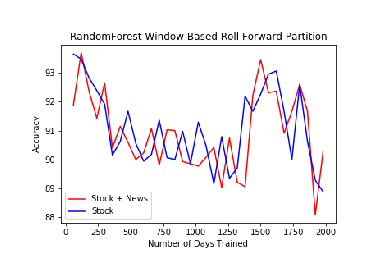
\includegraphics[width=10cm,height=10cm,keepaspectratio]{RandomForest_Window_Training_Acc.eps}
\caption{\label{fig:RandomForest_window_training} Random Forest Window Based Roll Forward Partition}
\end{figure}

\begin{figure}[H]
\centering
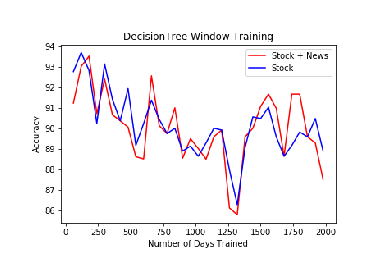
\includegraphics[width=10cm,height=10cm,keepaspectratio]{DecisionTree_Window_Training_Acc.eps}
\caption{\label{fig:DecisionTree_window_training} Decision Tree Window Based Roll Forward Partition}
\end{figure}

\begin{figure}[H]
\centering
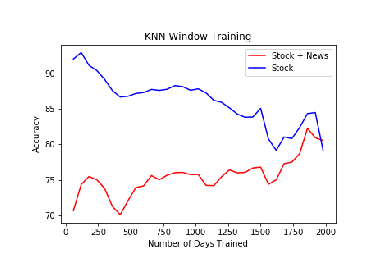
\includegraphics[width=10cm,height=10cm,keepaspectratio]{KNN_Window_Training_Acc.eps}
\caption{\label{fig:KNN_window_training} KNN Window Based Roll Forward Partition}
\end{figure}

From Figures~\ref{fig:XGBoost_window_training}, \ref{fig:RandomForest_window_training}, \ref{fig:DecisionTree_window_training} and  \ref{fig:KNN_window_training} it is observed that XGBoost has the highest accuracy(97 percent) followed by Random Forest (94 percent), Decision Tree (94 percent) and then KNN (91 percent) . All the algorithms except KNN are able to learn the Combined(Stock+News) dataset better than the dataset with only Stock features. 

\section{CONCLUSION}
This paper sought to introduce a way to combine news headlines and stock market features to predict the movement of stock market using machine learning and natural language processing techniques.

A different type of splitting the dataset was also used which produced an accuracy as high as 97 percent. This type of partitioning was done to provide an answer to the question of how many days prior to the day to be predicted needs to be considered for training the model.

The models also gave improved accuracy values on predicting the combined dataset as compared to the dataset which contained only stock features. This was observed in both the types of partitioning the data.

In the preprocessing of news, the usage of Tf-Idf as a way to filter out the stop words also gave improved results as seen by the the coherence score values. In future studies, an improvement which can be done to improve the text processing could be by using dimensionality reduction techniques like principal component analysis to the obtained numerical features of the news.

The accuracy can be further improved by reducing the time lag between news and stock market reactions. For example, in this paper, the time lag is of a day. If this is reduced to minutes or seconds and with better computational efficiencies and devices, the accuracy will definitely be improved.

The method used in this paper can be extended to a particular sectoral index or company by using an appropriate news dataset. Further clustering techniques can be applied to the output dataset so that instead of the direction, these clusters can be predicted. This would help in predicting drastic movement in markets. In a classical way, stock market has always been attributed as a time series data.Hence, many studies were conducted (\cite{time_series_1} and \cite{time_series_2}) to predict the price movements using time series models.

This paper gives insights about forecasting stock market movements using machine learning and natural language processing techniques and helps in the applying machine learning models to stock market trading in a novel way.



\medskip
\pagebreak

\begin{thebibliography}{9}

\bibitem{emh}
Fama, E. F., 1991. Efficient capital markets: Ii. The journal of finance 46 (5), 1575–1617.



\bibitem{text_1}
Nasseri, A. A., Tucker, A., \& de Cesare, S. (2015). Quantifying StockTwits semantic terms’ trading behavior in financial markets: An effective application of decision tree algorithms. Expert Systems with Applications, 42(23), 9192–9210. doi:10.1016/j.eswa.2015.08.008 


\bibitem{text_2}
Khadjeh Nassirtoussi, A., Aghabozorgi, S., Ying Wah, T., \& Ngo, D. C. L. (2015). Text mining of news-headlines for FOREX market prediction: A Multi-layer Dimension Reduction Algorithm with semantics and sentiment. Expert Systems with Applications, 42(1), 306–324. doi:10.1016/j.eswa.2014.08.004 
\bibitem{text_3}
Khadjeh Nassirtoussi, A., Aghabozorgi, S., Ying Wah, T., \& Ngo, D. C. L. (2014). Text mining for market prediction: A systematic review. Expert Systems with Applications, 41(16), 7653–7670. doi:10.1016/j.eswa.2014.06.009 


\bibitem{stock_1}
Chatzis, S. P., Siakoulis, V., Petropoulos, A., Stavroulakis, E., \& Vlachogiannakis, N. (2018). Forecasting stock market crisis events using deep and statistical machine learning techniques. Expert Systems with Applications, 112, 353–371. doi:10.1016/j.eswa.2018.06.032 


\bibitem{stock_2}
Weng, B., Ahmed, M. A., \& Megahed, F. M. (2017). Stock market one-day ahead movement prediction using disparate data sources. Expert Systems with Applications, 79, 153–163. doi:10.1016/j.eswa.2017.02.041 



\bibitem{stock_3}
Weng, B., Lu, L., Wang, X., Megahed, F. M., \& Martinez, W. (2018). Predicting short-term stock prices using ensemble methods and online data sources. Expert Systems with Applications, 112, 258–273. doi:10.1016/j.eswa.2018.06.016 




\bibitem{lda} 
David M. Blei and Andrew Y. Ng and Michael I. Jordan and John Lafferty (2003).Latent dirichlet allocation.Journal of Machine Learning Research.3,2003.doi:10.5555/944919.944937

\bibitem{tfidf_1}

HaCohen-Kerner, Y., Miller, D., \& Yigal, Y. (2020). The influence of preprocessing on text classification using a bag-of-words representation. PLOS ONE, 15(5), e0232525.doi:10.1371/journal.pone.0232525 

\bibitem{tfidf_2}
Gerlach, M., Shi, H., \& Amaral, L. A. N. (2019). A universal information theoretic approach to the identification of stopwords. Nature Machine Intelligence. doi:10.1038/s42256-019-0112-6 

\bibitem{tfidf_3}
Kim, S.-W., \& Gil, J.-M. (2019). Research paper classification systems based on TF-IDF and LDA schemes. Human-Centric Computing and Information Sciences, 9(1). 
doi:10.1186/s13673-019-0192-7 

\bibitem{random_forest} 
Breiman, L. (2001). Machine Learning, 45(1), 5–32. doi:10.1023/a:1010933404324 

\bibitem{xgboost}
Tianqi Chen and Carlos Guestrin. 2016. Xgboost: A scalable tree boosting system. In Proceedings of the 22nd acm sigkdd international conference on knowledge discovery and data mining. 785--794.  
doi:10.1145/2939672.2939785



\bibitem{time_series_1}
Sezer, O. B., \& Ozbayoglu, A. M. (2018). Algorithmic financial trading with deep convolutional neural networks: Time series to image conversion approach. Applied Soft Computing, 70, 525–538. doi:10.1016/j.asoc.2018.04.024 

\bibitem{time_series_2}
Sezer, O. B., Gudelek, M. U., \& Ozbayoglu, A. M. (2020). Financial time series forecasting with deep learning: A systematic literature review: 2005–2019. Applied Soft Computing, 106181. doi:10.1016/j.asoc.2020.106181 


\end{thebibliography}


\end{document}

\endinput
%%
%% End of file `elsarticle-template-harv.tex'.
